\section{Scaling Theory}
\subsection{Recap}
To recap; we are studying Gaussian theory, in particular $\phi^4$ theory of a magnet. This is mean field theory + quadratic fluctuations, which is exactly solvable, but can still give us insight.

We looked at correlation length associated to longitudinal and transverse fluctuations. We studied the effect of the transverse fluctuations/Goldstone mode, and below 2-$d$ the correlations die off and we have no LRO. This was the lower critical dimension. We will now study an upper critical dimension, which will turn out to be $d = 4$.

We look at the logarithm of the partition function:
\begin{equation}
    \ln Z = \frac{t}{2}\bar{m}^2 + \frac{u}{4}\bar{m}^4 + \int d^dx \left[\frac{1}{2}\kappa(\nabla \phi_l)^2 + \xi_l^{-2} \phi_l^2\right] + \int d^dx \left[\frac{1}{2}\kappa(\nabla \phi_t)^2 + \xi_t^{-2}\phi_t^2\right]
\end{equation}
The correlation lengths have the scaling:
\begin{equation}
    \xi_l = \begin{cases}
        \xi_0 t^{-1/2}  & t > 0 
        \\ (-2t)^{-1/2} & t < 0
    \end{cases}
\end{equation}
\begin{equation}
    \xi_t = \begin{cases}
        \xi_0 t^{-1/2} & t > 0 
        \\ \infty & t < 0
    \end{cases}
\end{equation}
The important observation for the transverse modes is below the phase transition, the $\xi_t\phi_t^2$ term is absent. We can do the integral by going into momentum space:
\begin{equation}
    \int d^dx \left[\frac{1}{2}\kappa(\nabla \phi_t)^2 + \xi_t^2\phi_t^2\right] = \int \frac{d^dq}{(2\pi)^d} \left[\frac{1}{2}\kappa (q^2 + \xi_t^{-2})\phi_t(q)^2\right]
\end{equation}
Then the partition function is:
\begin{equation}
    Z = Z_{MF}e^{-\ln\det(\kappa(q^2 + \xi_t^{-2}))}
\end{equation}
Where this comes from:
\begin{equation}
    Z = \int \mathcal{D}\phi_q e^{-\frac{1}{2}\int d^d q\kappa (q^2 + \xi_t^{-2})\phi_q^2}
\end{equation}
And then we take the Gaussian integral. Then computing the correlators from this result (dropping $\xi_t$ as we are $t < 0$);
\begin{equation}
    \avg{\phi_t(\v{q}), \phi_t(\v{q}')} = \frac{\delta_{\v{q} + \v{q}'}}{\kappa \v{q}^2} \implies \avg{\phi_t(\v{x})\phi_t(\v{x}')} = \int \frac{d^dq}{(2\pi)^d} \frac{e^{i\v{q} \cdot \v{x} - \v{x}'}}{\kappa \v{q}^2}
\end{equation}
from which we saw that:
\begin{equation}
    \lim_{x \to \infty}C(x = \abs{\v{x} - \v{x}'}) \propto \begin{cases}
        \text{Const} & d > 0
        \\ x^{2-d} & d < 2
        \\ \ln(x) & d =2 
    \end{cases}
\end{equation}
and found our lower critical dimension of $2$. 

\subsection{Massive Modes and Upper Critical Dimension}
We have the partition function of the longtitudinal modes:
\begin{equation}
    Z = Z_{MF}e^{-\ln\det(\kappa(q^2 + \xi_l^{-2}))}
\end{equation}
Let us look at the free energy, by taking the logarithm of $Z$:
\begin{equation}
    F = F_{MF} + \frac{1}{2}\int \frac{d^dq}{(2\pi)^d} \ln(\kappa(\v{q}^2 + t))
\end{equation}
Now looking at the heat capacity:
\begin{equation}
    C = -T\dpd[2]{F}{T} \sim -t\dpd[2]{F}{t}
\end{equation}
Looking at the contribution from the fluctuations:
\begin{equation}
    C \sim \int \frac{d^dq}{(2\pi)^d}\frac{1}{(\kappa q + t)^2} \stackrel{t \to 0}{\sim} \int_0^{1/a} dq \frac{q^{d-1}}{q^4} \sim a^{4d}
\end{equation}
we want to see how this integral behaves. For $d > 4$, we have the integral is well behaved at $q = 0$ and evaluates to $\sim a^{4d}$ as above. For $d < 4$, we need to keep the correlation length (else the integral does not converge) so:
\begin{equation}
    \int_0^{1/a}dq \frac{q^{d-1}}{(q^2 + \xi_l^{-2})} \sim \xi^{4-d}
\end{equation}
Plotting the heat capacity, we get:

\begin{figure}[htbp]
    \centering
    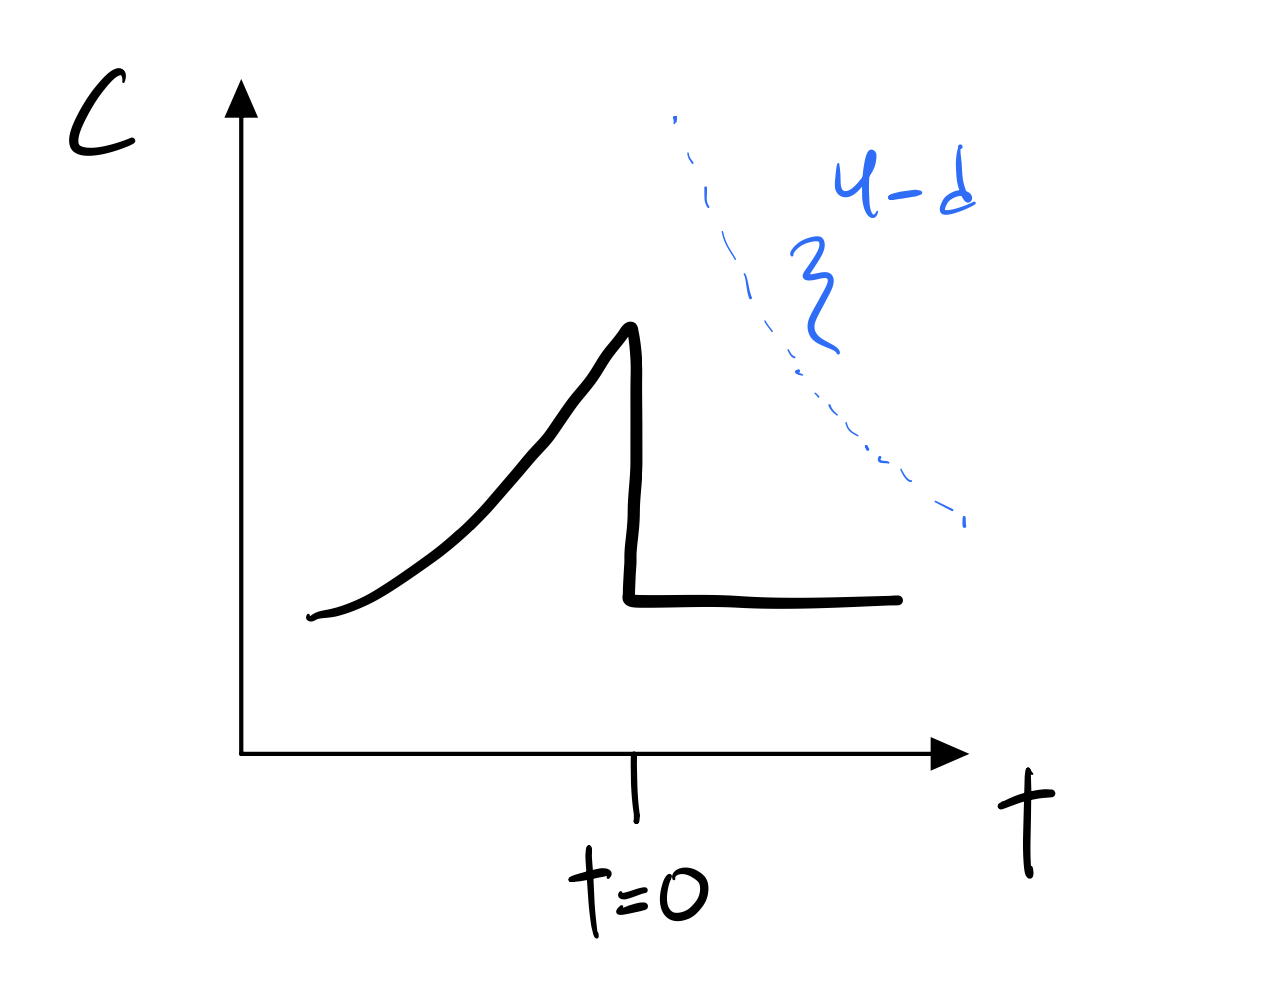
\includegraphics[scale=0.5]{Lectures/Figures/lec6heatcapacity.png}
    \caption{Plot of heat capacity for Gaussian theory.}
    \label{gaussian-heatcapacity}
\end{figure}

So, we see that Gaussian theory fails for $d < 4$. Why? We said MF theory + small fluctuations. If the effect of small fluctuations is benign, then we are happy. If the effect of small fluctuations is large, then we aren't happy; the theory is not self-consistent. Below $d < 4$, the failure of the integral to converge (and the rapid change in behaviour of physical quantities due to the fluctuations) tells us that the theory does not apply.

So below $d = 2$ we have no LRO, and above $d = 4$ we know that MFT + Gaussian fluctuations is ok. The interesting regime left to explore is $d = 2$ to $d = 4$. 

We also were studying the phase transition at $t = 0$ we can also ask about the magnitude of the fluctuations as we go away from the transitions.

In summary, we saw that the heat capacity from the mean field goes as $C_{MF} = \frac{1}{u}$ and the capacity of the fluctuations go as $C_{F} = \frac{\xi^{4-d}}{\kappa^2}$. The $\kappa$ is a microscopic parameter that characterizes the stiffness of the bare mode, with dimensional analysis from $\kappa \nabla^2$ telling us that $\kappa$ has a dimension of length square, i.e. $\kappa \sim \xi_0^{2}$. Thus:
\begin{equation}
    C_F \sim \frac{\xi_0^{4-d}\abs{t}^{-\frac{4-d}{2}}}{\xi_0^4} = \frac{1}{\xi_0^d}t^{-\frac{4-d}{2}}
\end{equation}
so indeed the $t$ piece diverges, but we have the $\xi_0$ piece characterizing the microscopic correlation length. So, if we have a system with a very long microscopic correlation length, we have to get very close to the transition $t = 0$ to see the divergence. This defines a temperature where the fluctuations where the fluctuations take over and the theory fails. This temperature is typically known as the \emph{Ginzburg temperature}. There are systems, typically superconductors, where the microscopic correlation length is very long. So, despite the fact that the correlations diverge, we have to get very close to the transitions to see these diverging correlations.

\subsection{Scaling Theory}
Is it going to be the case where I need a theory that calculates a new parameter for each fluctuating quantity? Or are they all related? Our proposal is the latter. Let us make this statements precise

\emph{Scaling theory:} Thermodynamic functions (e.g. the thermodynamic free energy $F$) are homogenous functions of scaled variables (e.g. $T, h$).

This hypothesis can be used to simplify the problem such that I may compute simple things. To be clear, we already had this in mean field theory. There, we looked at some (scaled) free energy which we viewed as the minimum of a power series expansion:
\begin{equation}
    f(t, h) = \min_m \left[\frac{t}{2}m^2 + \frac{u}{4}m^4 - hm\right]
\end{equation}
For example, this gave:
\begin{equation}
    f(t, h) = \begin{cases}
        -\frac{t^2}{4u} & h = 0, t < 0
        \\ -\frac{3}{4}\frac{h^{4/3}}{u^{1/3}} & h \neq 0, t = 0
    \end{cases}
\end{equation}
With a crossover line $h \sim \abs{t}^{3/2}$ below which we have the first behaviour, and above which we have the second.

\begin{figure}[htbp]
    \centering
    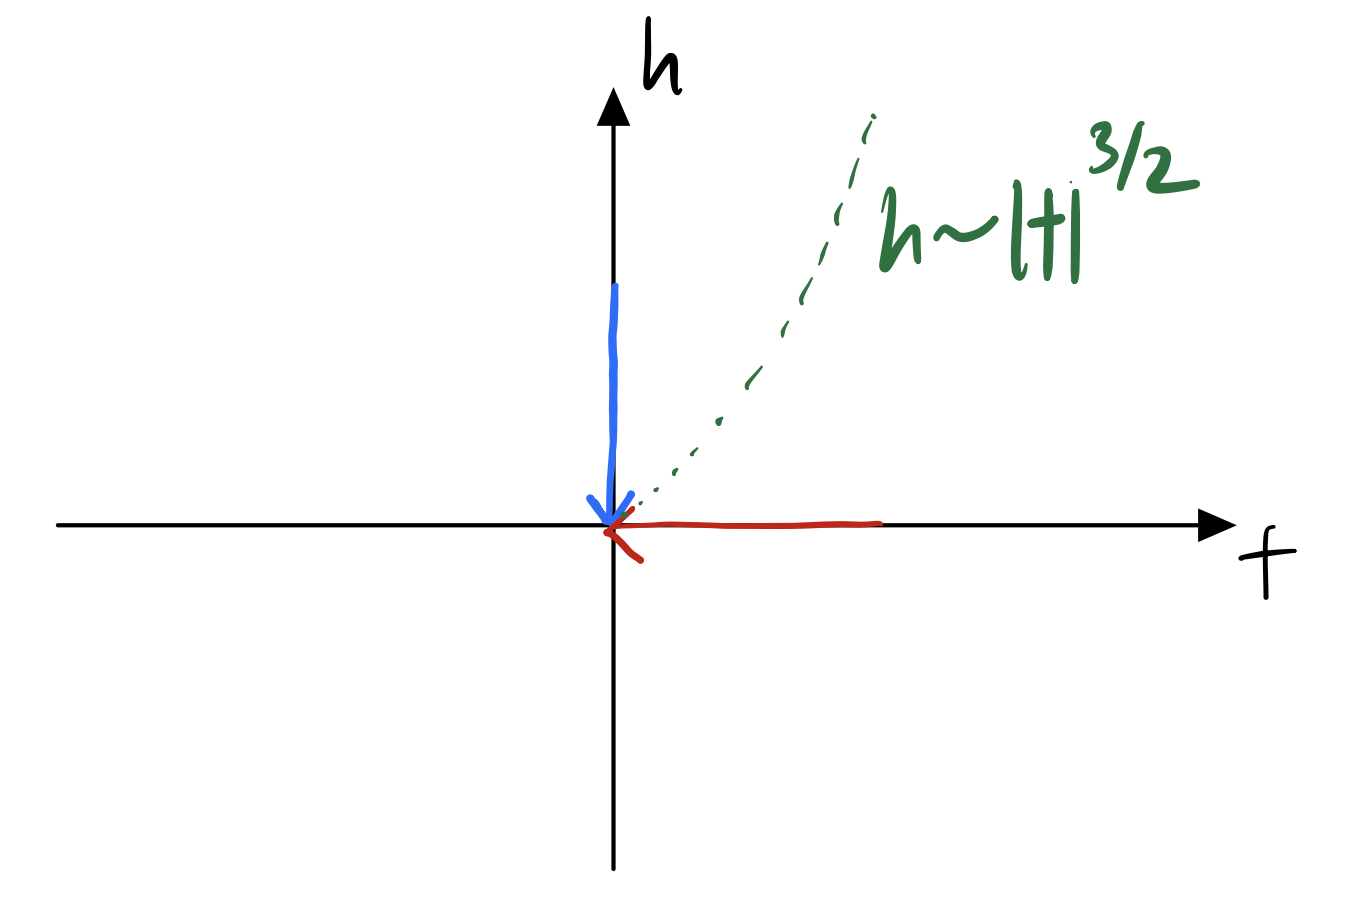
\includegraphics[scale=0.5]{Lectures/Figures/htcrossover.png}
    \caption{The free energy has a certain behaviour aloing the $h = 0$ and $t = 0$ lines. The crossover of these two behaviours occurs along $h \sim \abs{t}^{3/2}$.}
    \label{fig-htcrossover}
\end{figure}

Rewriting this in another way, We have:
\begin{equation}
    f(t, h) = \abs{t}^2g(h/\abs{t}^\Delta)
\end{equation}
where $g$ is a homogenous function of $h/\abs{t}^\Delta$. The previous calculations constrain $g$. E.g. at $g = 0$, we have:
\begin{equation}
    g(0) = -\frac{1}{4u}
\end{equation}
and
\begin{equation}
    g(x\to\infty) \sim x^{4/3}
\end{equation}
In the limit where $h$ is large, we also know the answer is independent of $t$, therefore if we have:
\begin{equation}
    f(t, h) = \abs{t}^2\left(\frac{h}{\abs{t}^\Delta}\right)^{4/3}
\end{equation}
the $t$-independence constrains $\Delta = 3/2$. 

In MF theory, we know precisely what $g$ is. In general with scaling analysis, we only know the asymptotic behaviour.

What we will do - we propose that there is a ``better theory'', where:
\begin{equation}
    f_{\text{sing}}(t, h) = \abs{t}^{2-\alpha}g(h/\abs{t}^\Delta)
\end{equation}
The singular component to the energy goes as:
\begin{equation}
    \begin{split}
        E_{\text{sing}} \sim \dpd{f}{t} &= (2-\alpha)\abs{t}^{1-\alpha}g(h/\abs{t}^\Delta) - \Delta h \abs{t}^{1-\alpha-\Delta}g'(h/\abs{t}^\Delta)
        \\ &= \abs{t}^{1-\alpha}\left((2-\alpha)g(h/\abs{t}^\Delta) - \Delta(\frac{h}{\abs{t}^\Delta})g'(h/\abs{t}^\Delta)\right)
    \end{split}
\end{equation}
where the term in brackets is another homogenous function, $g_E(h/\abs{t}^\Delta)$. To get the heat capacity, we take the derivative again:
\begin{equation}
    C_{\text{sing}} \sim -\dpd[2]{f}{t} = \abs{t}^{-\alpha}g_c(h/\abs{t}^\Delta)
\end{equation}
and we have the magnetization:
\begin{equation}
    m(t, h) = \dpd{f}{h} = \abs{t}^{2-\alpha-\Delta}g_m(h/\abs{t}^\Delta)
\end{equation}
now, as $h \to 0$, we have $g_m \to \text{const}$, and we identify the critical exponent $\beta = 2 - \alpha - \Delta$. For large arguments, we propose $g_M(x) \sim x^P$, then:
\begin{equation}
    m(t=0, h) \sim \abs{t}^{2-\alpha-\Delta}\left(\frac{h}{\abs{t}^\Delta}\right)^P
\end{equation} 
so by the $t$-independence argument, we have:
\begin{equation}
    2 - \alpha - \Delta = P\Delta
\end{equation}
and then:
\begin{equation}
    m(h) \sim h^{\frac{2-\alpha-\Delta}{\Delta}}
\end{equation}
so then we identify the exponent:
\begin{equation}
    \delta = \frac{\Delta}{2 - \alpha - \Delta} = \frac{\Delta}{\beta}
\end{equation}
whose measurement allows us to infer $\Delta$.

Why might this theory be true? Underlying this theory is a diverging correlation length, which gives you averaging, and is solely responsible for the singular fluctuations. The last thing we propose is that there is a correlation length $\xi$ that is hidden behind all of this phenomenology, where:
\begin{equation}
    \xi \sim \abs{t}^{-\nu}g_\xi(\frac{h}{\abs{t}^\Delta})
\end{equation}
where the divergence of $\xi$ is responsible for the rest of the behaviour we have analyzed. 

This is the hypothesis, and we have to work out this hypothesis in such a way that is self-consistently well behaved. The process we will go through (known as the \emph{renormalizaiton group}) will start with a Ginzburg-Landau theory, suggest there is a diverging length scale that is responsible for the phenomena, and then average that action on a characteristic length scale. We then scale. Then, supposing that the correlation length gets scaled, we can average again, and we want to force the averaging procedure to give us a function which is a homogenous function of the parameters. This is the process/constraint we put on scaling. We force the algebra to give us a scaling function like this. When we do this, there is a sequence of operations that will enable us to calculate these exponents. We can then check if the procedure is consistent, or not. This is what we will explore in future lectures.C